% v2-acmtog-sample.tex, dated March 7 2012
% This is a sample file for ACM Transactions on Graphics
%
% Compilation using 'acmtog.cls' - version 1.2 (March 2012), Aptara Inc.
% (c) 2010 Association for Computing Machinery (ACM)
%
% Questions/Suggestions/Feedback should be addressed to => "acmtexsupport@aptaracorp.com".
% Users can also go through the FAQs available on the journal's submission webpage.
%
% Steps to compile: latex, bibtex, latex latex
%
% For tracking purposes => this is v1.2 - March 2012
\documentclass{acmtog} % V1.2

%\acmVolume{VV}
%\acmNumber{N}
%\acmYear{YYYY}
%\acmMonth{Month}
%\acmArticleNum{XXX}
%\acmdoi{10.1145/XXXXXXX.YYYYYYY}

\acmVolume{28}
\acmNumber{4}
\acmYear{2009}
\acmMonth{September}
\acmArticleNum{106}
\acmdoi{10.1145/1559755.1559763}

\begin{document}

\markboth{V. F. Pamplona et al.}{Photorealistic Models for Pupil Light Reflex and Iridal Pattern Deformation}

\title{Approximating complex algorithms using Neural Networks} % title

\author{PETROS DEBESAY {\upshape and} KEVIN CHEN TRIEU
\affil{Shanghai Jiao Tong University}
% NOTE! Affiliations placed here should be for the institution where the
%       BULK of the research was done. If the author has gone to a new
%       institution, before publication, the (above) affiliation should NOT be changed.
%       The authors 'current' address may be given in the "Author's addresses:" block (below).
%       So for example, Mr. Fogarty, the bulk of the research was done at UIUC, and he is
%       currently affiliated with NASA.
}

\category{I.3.7}{Computer Graphics}{Three-Dimensional Graphics and Realism}[Animation]
\category{I.3.5}{Computer Graphics}{Computational Geometry and Object Modeling}[Physically based modeling]

\terms{Experimentation, Human Factors}

\keywords{Face animation, image-based modelling, iris animation, photorealism, physiologically-based modelling}

\acmformat{Petros Debesay, Kevin Chen Trieu. 2009. Photorealistic models for pupil light reflex and iridal pattern deformation.
{\em ACM Trans. Graph.} 28, 4, Article 106 (September 2009), 10 pages.\\
\doiline}

\maketitle

\begin{bottomstuff}
Manuel M. Oliveira acknowledges a CNPq-Brazil fellowship (305613/2007-3). Gladimir V. G. Baranoski acknowledges a
NSERC-Canada grant (238337). Microsoft Brazil provided additional support.
Authors' addresses: Sean Fogarty, (Current address) NASA Ames Research Center, Moffett Field, California 94035.
\end{bottomstuff}


\begin{abstract}
We introduce a physiologically-based model for pupil light reflex (PLR)
and an image-based model for iridal pattern deformation. Our PLR model
expresses the pupil diameter as a function of the lighting of the
environment, and is described by a delay-differential equation,
naturally adapting the pupil diameter even to abrupt changes in light
conditions. Since the parameters of our PLR model were derived from
measured data, it correctly simulates the actual behavior of the human
pupil. Another contribution of our work is a model for realistic
deformation of the iris pattern as a function of pupil dilation and
constriction. Our models produce high-fidelity appearance effects and
can be used to produce real-time predictive animations of the pupil and
iris under variable lighting conditions. We assess the predictability
and quality of our simulations through comparisons of modeled results
against measured data derived from experiments also described in this
work. Combined, our models can bring facial animation to new
photorealistic standards. Another contribution of our work is a model
for realistic deformation of the iris pattern as a function of pupil
dilation and constriction. Another contribution of our work is a model
for realistic deformation of the iris pattern as a function of pupil
dilation and constriction. Another contribution of our work is a model
for realistic deformation of the iris pattern as a function of pupil
dilation and constriction.
\end{abstract}

\section{Introduction}
Arguably, the most important features in facial animation are the eyes,
which are essential not only in directing the gaze of the
audience~\cite{BLR-2007}, but also in conveying the appropriate degree
of expression through pupil dilation and constriction movements. Hence,
for animations depicting close-up views of the face, natural-looking
eyes and pupil movements are highly desirable.
 
\begin{quote}
``Walt Disney once said to his animation team that the audience watches
the eyes and this is where the time and money must be spent if the
character is to act convincingly".
\end{quote}

Differently from most of the body, the human eye is subject to some
involuntary movements of the pupil, which are determined by ambient
illumination, drug action, and emotional conditions, among
others~\cite{BDDG-03}. Pupillary light reflex (PLR) is responsible for
the constriction of the pupil area in highly lit environments and for
its dilation in dimmed ones. PLR is an integral part of our daily
experience, and except for drug-induced action, is the single most
noticeable of such involuntary movements of the pupil.


\begin{table*}[t]
\tabcolsep22pt
\tbl{Summary of the  Main Mathematical and Physical Quantities Considered in the Development of the Proposed
Models}{%
\begin{tabular}{@{}ccc@{}}\hline
Symbol &{Description} &{Physical Unit} \\
\hline
$L_{b}$ & luminance & blondels (B) \\
$L_{fL}$ & luminance & foot-Lambert (fL) \\
$I_{l}$ & illuminance & lumens/$mm^2$  (lm/$mm^2$)\\
$R$ & light frequency & {Hertz (Hz)} \\
%% $\phi$ & retinal light flux & lumens  ({\it lm}) \\
%% $\bar{\phi}$ & retinal light flux threshold & lumens  ({\it lm}) \\
$D$ & pupil diameter & millimeters  ({\it mm}) \\
$A$ & pupil area & square millimeters  ($mm^2$) \\
$r_I$ & individual variability index & $r_I \in$ [0,1] \\
$t$ & current simulation time & milliseconds  ({\it ms}) \\
$\tau$ & pupil latency & milliseconds  ({\it ms}) \\
$x$ & muscular activity & none\\
$\rho_{i}$ & ratio describing the relative position & none \\
$\beta, \alpha, \gamma, k$ & constants of proportionality & none \\\hline
\end{tabular}}
\label{tab:symbols}
\begin{tabnote}
This is an example of table footnote. This is an example of table footnote. This is an example of table footnote.
This is an example of table footnote. This is an example of table footnote.
\end{tabnote}
\end{table*}

\begin{figure*}[t]
\centerline{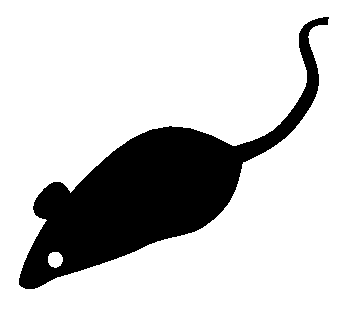
\includegraphics[width=11cm]{tog-sample-mouse}}
\caption{Comparison of the results predicted by our models against video
of a human iris. (left) One frame of an animation simulating the changes
in pupil diameter and iridal pattern deformation. (center) One frame
from a video of a human iris. (right) Graph comparing the measured pupil
diameters from each individual frame of a nine-second-long video
sequence (green line) against the behavior predicted by our model (red
line). The gray bars indicate the periods in which the light was kept on
and off. The complete video sequence and corresponding animation are
shown in the accompanying video.}
  \label{fig:videocomparison}
\end{figure*}

The human iris is a muscular tissue containing several easily
identifiable structures. Together, they define patterns that are
deformed as a result of changes in the pupil diameter. Although pupil
light reflex and iridal deformations could be animated using standard
computer graphics techniques, which in turn, may result in more
realistic and reproducible of these movements.

In this article, we present a physiologically-based model for realistic
animation of PLR. Our model combines and extends some theoretical
results from the field of mathematical biology~\cite{CDFKMS-06} with
experimental data collected by several {researchers} relating pupil
diameter to the intensity of environmental
light~\cite{BCHH:Collewijn:1988}. The resulting model produces
high-fidelity appearance effects and can be used to produce real-time
predictive animations of the pupil and iris under variable lighting
conditions (Section~\ref{sec:PLRValidation}). We model the iridal
pattern deformation process by acquiring a set of high-resolution
photographs of real irises at different levels of pupillary dilation and
by tracking their features across the set of images. By analyzing the
tracked positions, we obtained a simple analytical expression for the
iridal deformation pattern as a function of the pupil diameter
(Section~\ref{sec:patterndeformations}). To the best our knowledge, ours
is the first physiologically-based model for simulating pupil light
reflex presented in the graphics literature (the first model ever to
simulate individual variability in terms of PLR
sensitivity---Section~\ref{subsec:Variations}), as well as the first
model for iridal pattern deformation. Moreover, ours are the first
practical models (providing actual coefficient values) in the literature
for simulating the dynamics of the pupil and iris under variable
lighting conditions. We demonstrate the effectiveness of our approach by
comparing the results predicted by our models against photographs and
videos captured from real human irises
(Figures~\ref{fig:videocomparison} and 9). Table~\ref{tab:symbols}
summarizes the main mathematical and physical quantities used in the
derivation of the proposed models and which are considered throughout
this work.


\section{Related Work in Computer Graphics}
\label{sec:relatedwork}
%
\looseness-1A few researchers have addressed the issue of realistic
human iris synthesis. Lefohn et al. blend several textures created by an
artist, each containing some eye feature. Other image-based approaches
have been proposed by Cui et al., Wecker et~al., and Makthal and Ross.
Essentially, they decompose a set of iris images using techniques such
as principal component analysis, multiresolution and wavelets, and
Markov random fields, and recombine the obtained data to generate new
images of irises. Zuo and Schmid created a fiber-based 3D model of the
iris. Lam and Baranoski introduced a predictive light transport model
for the human iris, which computes the spectral responses of iridal
tissues described by biophysical parameters. Fran\c{c}ois et~al.
estimate iris height maps from gray-scale images. All these approaches
use stationary pupil sizes.

Sagar et al. developed an anatomically detailed model of the eye to be
used in a surgical simulator. In their model, Gaussian perturbations
were used to simulate the waviness of ciliary fibers and the retraction
of pupillary fibers during pupil dilation. Alternatively, depending on
the level of object manipulation, a texture mapping approach was used to
model the iridal appearance. It is worth noting, however, that their
goal was to achieve functional realism \cite{DS-02} as opposed to
physical or photorealism.

\section{Brief Overview of the Human Iris\break and Pupil}
\label{sec:biologicalreview}

The human iris has a diameter of about 12\,mm and forms a disc that
controls how much light reaches the retina. Under high levels of
lighting, the iris dilates, flattening itself and decreasing the pupil
size. Under low levels of illumination, it constricts, folding itself
and increasing the pupil area. The pupil diameter varies from 1.5\,mm to
8\,mm on average, and in general, it is not a perfect circle. Also, its
center may deviate from the center of the iris by an offset of up to
20\%. According to Newsome and Loewenfeld, there are no observable
differences in the iris regarding light-induced or drug-induced pupil
dilation/constriction.

The human iris is divided in two zones by the \emph{collarette}, a
delicate zig-zag line also known as the iris frill. The \emph{pupillary}
zone is bounded by the pupil, while the \emph{ciliary} zone extends to
the outer border of the iris. Each zone is characterized by a muscle.
The \emph{sphincter}, located in the pupillary zone, is a concentric
muscle that constricts to decrease the pupil size. The \emph{dilator},
found in the ciliary zone, is a radial muscle that constricts to
increase the pupil size. These two muscles overlap at the collarette.

The sphincter and dilator muscles are independently connected to the
autonomous nervous system (ANS) and the pupil size results from a
balance of the separately incoming stimuli to the two
muscles~\cite{Dod-1900}. The ANS conducts the pupillary light reflex and
\emph{hippus} neural actions. Hippus are spontaneously irregular
variations in pupil diameter, which can essentially be characterized as
random noise in the 0.05 to 0.3~Hz frequency range. In PLR, when light
reaches the retina, neural signals are sent to the brain, which sends
back a signal for closing or opening the pupil. Thus, PLR can be modeled
in two phases: perception, and after some time delay, adjustment.

\section{Models of Pupil Dynamics}
\label{sub:models_of_pupil_dynamics}

The pupillometry literature describes several models built around
experiments designed to measure the values of some parameters as a
function of incident light intensity. Link and Stark performed a study
where a light source was placed in front of the subjects' irises and, by
varying the intensity and frequency of the light, they measured the
pupillary latency (the time delay between the instant in which the light
pulse reaches the retina and the beginning of iridal reaction):
\begin{eqnarray}
  \tau(R,L_{fL}) & = & 253 - 14\,{{ln}}(L_{fL}) + 70 R - 29\, R\, {{ln}}(L_{fL}),
  \label{eq:Link_n_Stark}
\end{eqnarray}
where $\tau$ is the latency in milliseconds, $L_{fL}$ is the luminance
measured in foot-Lamberts (fL), and $R$ is the light frequency measured
in Hz.

Other similar models predict an average pupil size as a function of the
light intensity using a few experimental measurements~\cite{DC-1901}.
Among those, the most popular one is the Moon and Spencer model, which
is expressed as:
\begin{equation}
\label{eq:moon}
 D = 4.9 - 3 {{tanh}}[0.4 ({{log}}_{10}(L_{b}) - 0.5)],
\end{equation}
where the pupil diameter, $D$, varies from 2 to 8~mm, and $L_{b}$ is the
background luminance level expressed in blondels, varying from $10^5$
blondels in sunny days to $10^{-5}$ blondels in dark nights. $tanh$ is
the hyperbolic tangent.

\subsection{Physiologically-Based Models}
\label{subsub:theoretical_models}
%
In Mathematical Biology and related fields, models based on
physiological and anatomical observations were derived to express the
relationships among the pupillary action variables without relying on
quantitative experimental data. For example, Usui and Stark proposed a
parametric model of the iris to describe the static characteristics of
pupil response to light stimuli, and to explain its random fluctuations
in terms of probability density functions. Recently, Tilmant {et al.}
proposed a model of PLR based on physiological knowledge and guided by
experiments. Although they have obtained plausible results, Tilmant {et
al.}\ have recommended the use of another physiologically-based model to
more accurately monitor pupillary dynamics, namely the time-dependent
model developed by Longtin and Milton.

Longtin and Milton define the efferent neural signal $E(t)$ arriving at the iris per unit of time $t$,
as:
\begin{equation}
\label{eq:et}
    E(t) = \beta \; {{ln}} \left[ \frac{ \phi(t-\tau) }{ \bar{\phi} } \right],
    \label{eq:efferent_neural_signal_1}
\end{equation}
where $\beta$ is a constant of proportionality and $\phi$ is the retinal
light flux measured in lumens and defined by Stark and Sherman as $\phi
= I_{l}A$: illuminance ($I_{l}$, in lumens/$mm^2$) times the pupil area
($A$, in $mm^2$). $\tau$ is the latency, and $\bar{\phi}$ is the retinal
light level threshold (the light level below which there is no change in
the pupil area). The notation $\phi(t-\tau)$ indicates that the current
effect depends on the retinal light flux at a time $\tau$ milliseconds
in the past. As the efferent neural signal reaches the iris, it induces
some muscular activity $x$ that may cause the pupil to dilate or
constrict. According to Partridge and Benton, the relationship between
$E(t)$ and $x$ can be approximated by:
\begin{equation}
E(t) \tilde{=} k \left( \frac{dx}{dt} + \alpha x \right),
    \label{eq:efferent_neural_signal_2}
\end{equation}
where $k$ is a proportionality factor and $\alpha$ is a rate constant
that depends on the definition and units of $x$ used in the model.
Longtin and Milton combine Equations~(\ref{eq:efferent_neural_signal_1})
and (\ref{eq:efferent_neural_signal_2}) as:
\begin{equation}
  \label{eq:ativ}
  \frac{dx}{dt} + \alpha x = \gamma \; {{ln}} \left[ \frac{ \phi(t-\tau) }{ \bar{\phi} } \right].
  \label{eq:delay_differential}
\end{equation}
They express the pupil area as $A = f(x)$ and use the inverse $f^{-1}(A)
= g(A) = x$ to remove $x$ from Equation~(\ref{eq:delay_differential}).
In their paper, Longtin and Milton use a Hill function \cite{Duc-2002}
(Equation~\ref{eq:Hill_function}) as the function $f$, since it can
approximate the elasto-mechanical properties of the iris during the
pupillary activity:
\begin{equation}
\label{eq:area}
  A = f(x) = \frac{\Lambda\theta^n}{\theta^n+x^n} + \Lambda'.
  \label{eq:Hill_function}
\end{equation}
Here, $\Lambda'$ and $\Lambda + \Lambda'$ are, respectively, the minimum
and the maximum pupil areas, and $\theta$ is the value of $x$
corresponding to the average pupil area. Longtin and Milton's model then
becomes:
\begin{equation}
  \frac{dg}{dA}\frac{dA}{dt} + \alpha g(A) = \gamma \; {{ln}} \left[ \frac{ \phi(t-\tau) }{ \bar{\phi} }
\right],
\label{eq:longtin}
\end{equation}
where
\begin{equation}
  g(A) = x = \sqrt[n]{ \frac {\Lambda \theta^n} { A - \Lambda'} - \theta^n }.
\label{eq:inverseHill}
\end{equation}

An S-shaped curve similar to the Hill function has been described in the
physiologically-based model of Usui and Stark to approximate the pupil
diameter of an average individual under static illumination conditions.

\section{The Proposed Physiological-Based Model}
\label{sec:proposed_model}
%
The model of Moon and Spencer (Equation~(\ref{eq:moon})) is based on a
set of discrete measurements and approximates the response on an average
individual under various lighting conditions. Their measurements were
made after the pupil size had stabilized for each illumination level,
and therefore, their model does not describe the pupil behavior outside
the equilibrium state. Moreover, pupil size, latency, constriction, and
redilation velocities tend to vary among individuals exposed to the same
lighting stimulus~\cite{GPMBH-2005}. We remark that such variations are
not captured by the model of Moon and Spencer.

Longtin and Milton's model (Equation~(\ref{eq:longtin})) is time
dependent and adaptive, with the potential to handle abrupt lighting
changes. It is a theoretical model, and unfortunately, Longtin and
Milton did not provide the values for the various parameters in their
model (\emph{i.e.}, $\gamma$, $\alpha$, $\theta$, $n$, $\bar{\phi}$), as
these, in principle, depend on the abstract notion of iridal muscular
activity $x$, as well as on the use of the Hill function. The use of
incorrect parameter values will not produce realistic results and may
cause Equation~(\ref{eq:longtin}) to not converge.

Starting from Longtin and Milton's and from Moon and Spencer's models,
we derive a practical model that predicts the pupil diameter for the
nonequilibrium case based on experimental data
(Section~\ref{subsec:DynamicCase}). In Section \ref{subsec:Variations},
we show how we can extend this basic model to take individual
variability into account.

\subsection{Equilibrium Case}
\label{subsec:EquilibriumCase}
Under constant lighting conditions, the pupil area in Longtin and
Milton's model will converge to an equilibrium state, where:
\begin{eqnarray*}
  \frac{dg}{dA}\frac{dA}{dt} = 0.
  \label{eq:longtinArea}
\end{eqnarray*}
%
Under such a circumstance, and assuming there is no occurrence of
hippus, $\phi$ becomes time invariant. Also, recall that
${{ln}}(m/n)={{ln}}(m) - ln(n)$, and therefore, one can rewrite Longtin
and Milton's model (Equation~(\ref{eq:longtin})) for the equilibrium
case as:
\begin{equation}
 \alpha g(A) = \gamma \; ({{ln}}(\phi) - {{ln}}(\bar{\phi})).
 \label{eq:Milton_for_experiment}
\end{equation}
%
In turn, the Moon and Spencer model can be rewritten as
\begin{eqnarray*}
  \left(\frac{D - 4.9}{3} \right) = \left[0.4 \left( \frac{ln}{(L_{b})}ln(10) - 0.5 \left(\frac{ln}{(10)}ln(10)\right)
\right)\right],
  \label{eq:moonAndSpencerRewrote}
\end{eqnarray*}
and since the hyperbolic tangent is an odd function, we can rewrite this equation as:
\begin{equation}
  -2.3026 \; {{atanh}} \left(\frac{D-4.9}{3}\right) = 0.4 ({{ln}}(L_{b}) -1.1513),
\label{eq:moonChanged}
\end{equation}
where ${{atanh}}$ is the arc-hyperbolic tangent. Comparing Equations~(\ref{eq:Milton_for_experiment}) and
(\ref{eq:moonChanged}), in order for  Longtin and Milton's model to fit the response of Moon and Spencer's average
subject under  equilibrium conditions, one has:
\begin{eqnarray}
\label{eq:moonsEqualsLongtins1}
 -2.3026 \; {{atanh}} \left(\frac{D-4.9}{3}\right) & \approx & \alpha g(A) \\
\label{eq:moonsEqualsLongtins2}
 0.4 ( {{ln}}(L_{b}) -1.1513)  & \approx &  \gamma ({{ln}}(\phi) - {{ln}}(\bar{\phi})).
\end{eqnarray}
%
From Equation~(\ref{eq:moonsEqualsLongtins2}) we can estimate the value
of the parameter $\gamma$. One should note that $L_b$ is expressed in
blondels while $\phi$ is given in lumens. Although, in general one
cannot convert between two photometric quantities, this can be done
under some well-defined situations. Since Moon and Spencer's data were
collected with the subject seated before a large white screen of uniform
intensity which covers most of their field of view, we assume that the
light reaching a person's pupil has been reflected by a perfect
(Lambertian) diffuse surface. Recall that an ideal (lossless) diffuse
reflector returns all of the incident flux so that its reflectance $\rho
= 1$ and its BRDF $f = 1/\pi$. For such a reflector, $1$~blondel $=
10^{-6}$ lumens/mm$^2$.

Since the light flux, $\phi$, depends on the area of the pupil, in order
to estimate $\gamma$, we first evaluate the left-hand side of
Equation~(\ref{eq:moonsEqualsLongtins2}) for the entire range of
illumination covered by Moon and Spencer's model: $L_b \in [10^{-5},
10^{5}]$ blondels. For each value of $L_b$, we then use
Equation~(\ref{eq:moon}) to estimate $D$, from which the pupil area $A =
\pi(D/2)^2$, and then $\phi$, are computed. The retinal light level
threshold $\bar{\phi} = 4.8118\times10^{-10}$ lumens was obtained using
the pupil diameter $D_t=7.8272$~mm, predicted by Equation~\ref{eq:moon}
for $L_b = 10^{-5}$ blondels ($\bar{\phi} = \pi(7.8272 / 2)^2~mm^2
\times 10^{-5} 10^{-6}$ lumens/mm$^2$). Using the tabulated data for the
left-hand side of Equation~(\ref{eq:moonsEqualsLongtins2}) and the
conversion scheme just described, we get the following fitting:
\begin{equation}
  0.4 ( {{ln}}(L_{b}) -1.1513)      \approx  0.45 \; ({{ln}}(\phi) - {{ln}}(\bar{\phi})) -5.2,
 \label{eq:approx_log_terms}
\end{equation}
whose quality of approximation is illustrated in
Figure~\ref{fig:Longtin_v_Moon_right_and_comparison} (left). The
vertical axis of the graph (scaled muscular activity) represents $\alpha
g(A)$, where $g(A) = x$ is the muscular activity. The extra constant
$-5.2$ translates the function on the right-hand side of
Equation~\ref{eq:moonsEqualsLongtins2} vertically, improving the
fitting. Given Equation~(\ref{eq:approx_log_terms}), we can replace
$g(A)$ with $M(D)$ (Equation~(\ref{eq:moonsEqualsLongtins1})), with
$\alpha = -2.3026$, where $M(D)$ is given by:
\begin{equation}
  M(D) = {{atanh}} \left( \frac{D-4.9}{3} \right).
  \label{eq:our_function_for_elasto_mechanical_prop}
\end{equation}
Thus, the equilibrium situation can be expressed by
Equation~(\ref{eq:our_model}). As expected, it approximates Moon and
Spencer's function (Equation~(\ref{eq:moon})) for the pupil diameter of
the average subject quite well. The absolute value of the difference
between Equations~(\ref{eq:moon}) and (\ref{eq:our_model}) is under
$2\%$ over the entire range of $[10^{-5}, 10^{5}]$ blondels
(Figure~\ref{fig:Longtin_v_Moon_right_and_comparison} right).
\begin{equation}
\label{eq:our_model}
  2.3026 \; M(D)  =  5.2 - 0.45 \; {{ln}} \left[\frac{\phi}{\bar{\phi}} \right]
\end{equation}
%
\begin{figure}[t]
\centerline{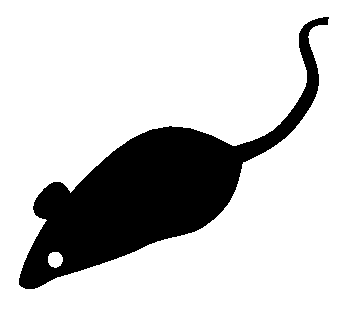
\includegraphics[width=7cm]{tog-sample-mouse}}
\caption{High-quality fittings: (left) Both sides of
Equation~\ref{eq:approx_log_terms}. (right) Equations~\ref{eq:moon} and
\ref{eq:our_model}, whose difference in absolute values is under $2\%$
over the entire range $[10^{-5}, 10^{5}]$ blondels.}
    \label{fig:Longtin_v_Moon_right_and_comparison}
\end{figure}
%
\subsection{The Dynamic Case}
\label{subsec:DynamicCase}
%
Equation~(\ref{eq:our_model}) cannot be used to describe the evolution
of the pupil diameter in time as a function of instantaneous variations
of the light intensity arriving at the pupil. Nevertheless, the obtained
constants are still valid for the dynamic case, since the equilibrium is
just a special case of the more general pupil behavior, for which the
constants should also hold.

In general, one cannot take an equation obtained for equilibrium and
generalize it to the dynamic case. In our model, however, this is
possible because of the following constraints:
\begin{enumerate}
\item[(1)] $g(A)$ and $M(D)$ have no explicit time dependence;
\item[(2)] the range of values assumed by $A$ (or $D$) is the same for
both the equilibrium and the nonequilibrium cases;
\item[(3)] there is a one-to-one mapping between $A$ and $D$.
\end{enumerate}

By introducing time in Equation~(\ref{eq:our_model}), we obtain a delay differential equation that
corresponds to our solution for the dynamic case:
\begin{equation}
\label{eq:dTEval}
  {{dt}}_{c} = \frac{T_{c} - T_{p}}{S} \quad
  {{dt}}_{d} = \frac{T_{c} - T_{p}}{3S},
\end{equation}
where $T_{c}$ and $T_{p}$ are respectively the current and previous
simulation times (times since the simulation started) measured in
milliseconds, $S$ is a constant that affects the constriction/dilation
velocity and varies among individuals. The higher the $S$ value, the
smaller the time step used in the simulation and, consequently, the
smaller the pupil constriction/dilation velocity.


Figure~4 shows pupil diameter values corresponding to Moon and Spencer's average
subject simulated using Equation~(16) considering some abrupt changes in the environment luminance.
For this example, our results are compared to results provided by the static models of Moon and Spencer
(Equation~(\ref{eq:moon})) and of De Groot and Gebhard.
%

\subsection{Modeling Individual Differences}
\label{subsec:Variations}

While Equation~(16) simulates dynamic pupil behavior, it only does so
for the average individual represented by the Moon and Spencer model.
There are, however, substantial differences in the way pupils from
different individuals react to a given light stimulus. Such variations
include differences in diameter~\cite{google}, latency, and constriction
and redilation velocities. In order to simulate individual differences,
we cannot just arbitrarily change the parameter values of our model, as
Equation~(16) may not converge.

Figure~3 shows the original data used by Moon and Spencer. The curve
$C_m$ (shown in black), was obtained by converting the values of $L_b$
in the range of $[10^{-5}, 10^{5}]$ blondels to lumens (see
Section~\ref{subsec:EquilibriumCase}) and then using
Equation~(\ref{eq:our_model}) to compute the corresponding pupil
diameter values used for plotting. The top and bottom curves, $C_t$ and
$C_b$, respectively, define an envelope containing all pupil diameter
values used by Moon and Spencer. $C_b$ was obtained by fitting a 5
degree polynomial to 11 of the smallest pupil diameter values along the
entire luminance range. Likewise, $C_t$ was obtained by fitting a 5
degree polynomial to 11 of the largest pupil diameter values. We treat
$C_b$, $C_m$, and $C_t$ as isocurves $C(p)$ for some parameter $p \in
[0,1]$, so that $C(0) = C_b$, and $C(1) = C_t$. We then model individual
differences by associating to each individual $I$, an index $r_I \in
[0,1]$, which corresponds to an isocurve, $C(r_I)$. This index can be
randomly generated or, alternatively, it can be recovered from
experimental data as described in Section~\ref{sec:PLRValidation}. To
avoid convergence problems and still achieve the results corresponding
to isocurve $C(r_I)$, we rewrite $C_t$ and $C_b$, respectively, as new
functions $C_{tD}$ and $C_{bD}$ of the pupil diameter:
\begin{eqnarray}
\label{eq:ctD}
  C_{tD}(D) &=& \,{-}\,0.013 D^5  +  0.322 D^4 - 3.096 D^3\nonumber\\
              &&\,{+}\,13.655 D^2 - 25.347 D + 18.179\\
\label{eq:cbD}
  C_{bD}(D) &=& \,{-}\,5.442 D^5 + 1.387 D^4 - 1.343 D^3\nonumber\\
              &&\,{+}\,6.219 D^2 - 1.317 D   + 1.219.
\end{eqnarray}
%

\looseness-1In order to obtain $C_{tD}$, we evaluate the functions $C_m$
and $C_t$ for $L_b$ in the range $[10^{-5}, 10^5]$ blondels, creating
ordered pairs of diameter values $(D_m, D_t) = (C_m(L_b), C_t(L_b))$.
Given enough of these pairs, we fit a curve expressing $D_t$ as a
function of $D_m$ (or $D$ for short). The resulting curve is $C_{tD}$
(Equation~(\ref{eq:ctD})). The case of $C_{bD}$ is similar. The final
pupil diameter at any time is then obtained solving Equation~16 for $D$
and then evaluating:
\begin{equation}
\label{eq:isocurve}
D_{final} = C_{bD}(D) + (C_{tD}(D) - C_{bD}(D)) r_I.
\end{equation}
We have adopted this solution due to its simplicity and generality: we
can easily replace the curves $C_{bD}(D)$ and $C_{tD}(D)$ with new ones,
covering new data as they become available, or representing other models
(e.g., De Groot and Gebhard). Since the relative distances of $C_m$ to
$C_b$ and $C_t$ vary for different values of $D$, no value of $r_I$ will
exactly recover $C_m$. This is not a problem, however, as $C_m$
corresponds to the average subject. Other parameterizations are
possible, including ones that interpolate $C_m$ for a given value of
$r_I$.

Although our model properly simulates the elastic behavior of the iris
muscular activity during changes in lighting conditions, it does not
model hippus (Equation~16 will converge to some pupil diameter value if
the lighting conditions remain constant). As random fluctuations whose
causes are still unknown, it is currently not possible to define a
physiologically-based model for hippus. We visually approximate the
hippus effect by adding small random variations to the light intensity
(between $-10^{0.3}$ and $10^{0.3}$ blondels), to induce small
variations in the pupil diameter (of the order of 0.2 mm), in the
frequency range of 0.05Hz to 0.3Hz. This significantly improves the
realism of the resulting simulations and animations. According to Usui
and Stark, the standard deviation of the noise corresponds to
approximately 10\% of the pupil diameter.


\subsection{The PLR Model Validation}
\label{sec:PLRValidation}
%
In order to validate our PLR model under nonequilibrium conditions and
to show that it is capable of representing individual variability, we
performed some qualitative comparisons between actual pupil behavior and
the results of simulations produced by our model. For this, we captured
videos of normal subjects presenting significantly different light
sensitivities (different PLR responses), while a light was turned {on}
and {off} several times. Since pupil constriction is bigger when both
eyes are stimulated, the subjects kept both eyes opened. To avoid
fatigue and habituation of the iris, in each experiment we recorded less
than one minute of video per subject.
\begin{itemize}
\item The image texel size of surface textures that represent 3D
elements (e.g. forest) should vary with distance, but should not match
true perspective (\emph{texel size} in Section~3.2, Texture Gradients).
\item The image space distribution of texel elements of 3D textures
(e.g. forest) should mimic one that would result from the projection of
homogeneously distributed surface elements (\emph{texel density} in
Section~3.2, Texture Gradients).
\item Image space texel spacing of 3D textures should ensure that texels
overlap, especially in steep areas (\emph{texel occlusion} in
Section~3.2, Texture Gradients).
\item Fall lines follow essential structures of terrain. They act as
surface contours, and are used by panorama artists to paint cliff and
snow textures (\emph{fall lines} in Section~3.2, Surface Contours).
\item Fall lines are used as imaginary lines along which tree strokes
are placed, acting as texture \emph{meta-strokes} (\emph{meta-strokes}
in Section~3.2, Surface Contours).
\item Shading tone should have a good distribution of light, medium, and
dark values (\emph{shading} in Section~3.2, Shading).
\item Light position should be placed so that the rendering of the
terrain exhibits a good balance of light and shade, as seen from the
selected viewpoint (\emph{light direction} in Section~3.2, Shading).
\item For extended terrain areas, indicating silhouettes, especially
between occluding hills, is useful (\emph{silhouettes} in Section~3.2,
Silhouettes).
\item Water surfaces should reflect the environment (\emph{water
textures} in Section~3.3, Brushstroke Colors).
\item Geometry should be emphasized by use of vertical exaggeration
(\emph{vertical exaggeration} in Section~3.4).
\end{itemize}

We computed the pupil diameters of the subjects at each frame of the
video sequences. Lighting measurements made during video capture were
used as input to our PLR model for simulating pupil behavior. The pupil
diameters resulting from these simulations were then compared to the
pupil diameters computed at individual video frames. Note that the
simulated results are not expected to quantitatively match the observed
ones, but rather be in qualitative agreement with observed behavior.

The videos were captured using a Cannon ELURA2 miniDV camcorder (NTSC,
720$\times$576 pixels) with progressive scan, connected to a PC through
a firewire connection. We kept the room's light dimmed so that the
subjects' pupils could dilate naturally to some extent, but not so dark
that we could not see the pupils in the individual video frames. Because
of these constraints, we used two subjects (both males) with light eyes
(a 24-year-old with green eyes, and a 26-year-old with blue eyes). For
each frame, the pupil diameters were estimated from the set of dark
pixels (pupil area $P_{area}$) inside a specified rectangle containing
solely the subject's pupil and part of the iris (Figure~5). Given
$P_{area}$, the pupil diameter was obtained (assuming the pupil is a
circle) as $d = 2(\sqrt{P_{area}/\pi})$ pixels. The conversion from
pixels to millimeters was performed considering a typical iris diameter
of 12mm. According to our experience, computing the pupil diameter as
described produces more accurate results than computing it as the number
of pixels in the largest straight segment in the set of dark pixels (the
pupil).

Since the video frames were captured at approximately 30Hz, in practice
no variation is expected between the pupil diameters in neighbor frames
under constant illumination, even in the presence of hippus. Thus, we
estimated the average error in the computed pupil diameters to be
approximately 0.1mm by computing the average difference between
estimated pupil diameters for neighbor frames. Based on the video
sequences, we set $S = 600$ (Equation~(\ref{eq:dTEval})) for the two
subjects in all experiments, as this value made their simulated
constriction velocities approximate the ones in the video sequences. We
empirically set the frequency of the two light sources used in our
experiments to $R = 0.4$Hz, a value that made the latency estimated by
Equation~(\ref{eq:Link_n_Stark}) approximate the latency observed in the
video frames.

To evaluate the quality of our simulations, we performed experiments
with both subjects using two different kinds of light sources to induce
pupil constriction: a small flashlight and a 100-watt incandescent white
light bulb. For light measurements, we used an LD-200 Instrutemp digital
lux meter (precision $\pm3\%$, frequency 2\,Hz).

\subsubsection{The Flashlight Experiments}
\label{sec:first_flashlightExperiment}

In these experiments, we used a light source to induce significant
changes in the subjects' pupil diameters without introducing
considerable changes in the lighting conditions of the environment. For
this purpose, we used a small flashlight powered by a single AAA battery
(1.5 Volt) kept at about 20cm from the subject's right eye and pointed
at it. Given the small area illuminated by the flashlight as well as its
reduced power, the readings from the lux meter were very sensitive to
even small changes in the relative position and orientation of the
flashlight with respect to lux meter sensor. Thus, we decided to run two
simulations using the recorded data: (1) considering the light intensity
estimated using Equation~(\ref{eq:moon}), and (2) considering the
readings from the lux meter. These two experiments are explained next.

In this experiment, we used the Moon and Spencer equation
(Equation~(\ref{eq:moon})) to solve for the light intensities during the
{on} and {off} states of the flashlight, based on the measured pupil
diameters (from the video). Since the Moon and Spencer function (curve
$C_m$ in Figure~3) represents the pupil behavior of an average
individual, we estimated the {on} ({off}) light intensity as the average
of the computed {on} ({off}) intensities for both subjects. Using this
procedure, we obtained estimates of $10^{1.1}$~blondels when the
flashlight was on, and $10^{-0.5}$~blondels when the flashlight was off.
Given the average luminance value for the {on} ({off}) state and the
{corresponding} pupil diameter for a given subject, we used
Equation~(\ref{eq:isocurve}) to estimate the $r_{I_{on}}$
($r_{I_{off}}$) index for that subject. The subject's final $r_I$ index
was computed as the average between his \smash{$r_{I_{on}}$} and
\smash{$r_{I_{off}}$} indices. Using this procedure, we obtained $r_I =
0.4$ for the green-eye subject and $r_I = 0.03$ for the blue-eye
subject.

Figure~6 shows the actual pupil diameter measurements performed on a
frame-by-frame basis along 9-second-long sequences captured for each
subject. The green ``+" marks on top represent the measurements for the
green-eye subject, while the blue ``x" marks show the measurements of
the blue-eye subject. This example illustrates the intersubject
variability in terms of light sensitivity and shows the ability of our
model to appropriately represent such individual differences. The
vertical dotted lines delimit the intervals in which the flashlight was
kept on and off for each subject.
%Note that the duration of these intervals varied as the video sequences were acquired.
The solid and dashed lines represent the simulated results produced by
our model for the green-eye and blue-eye subjects, respectively, and
closely agree with the actual measured values. These curves were
produced automatically from Equations~(16) and~(\ref{eq:isocurve}), on
top of which we added small random variations (hippus effect) as
described in the previous section. The accompanying video shows
side-by-side comparisons of our simulated results and videos captured
for the two subjects.
 
\paragraph{The second flashlight experiment}
In this experiment, we used the readings provided by the lux meter for
the {on} and {off} states of the flashlight. These illuminance values
were 350lux\footnote{$1~{{lux}} = 1~{{lumen}} /m^2$.} and 90lux,
respectively. One should recall that in such a setup, small changes in
the position and orientation of the subject's head produce changes in
the illuminance at the pupil. Therefore, these values are only
approximations to the actual illuminance reaching each subject's lit
eye. Given the illuminance values and the subjects' corresponding pupil
diameters estimated from the video frames, we obtained the actual
pupil's luminous flux (in lumens) at the two flashlight states, for each
individual. These values were then converted to blondels according to
the assumption described in Section~\ref{subsec:EquilibriumCase}. We
then used Equations~(16) and~(\ref{eq:isocurve}) to estimate their
corresponding $r_I$ indices (by averaging \smash{$r_{I_{on}}$} and
\smash{$r_{I_{off}}$}), obtaining $r_I = 0.54$ for the blue-eye subject
and $r_I = 0.92$ for the green-eye subject. Figure~7 compares the actual
pupil measurements (same as in Figure~6) with the results simulated by
our model using the lux meter readings as input. The differences between
the simulated curves shown in Figures~6 and 7 are primarily due to the
added random noise (hippus).


\subsubsection{The 100-Watt Lightbulb Experiment}
\label{sec:luxMeterExperiment}
For this experiment we used a more stable light source to induce pupil
constriction: a spot with a 100-watt incandescent white lightbulb, kept
at about one meter in front and one meter to the right of the subject's
head. This setup allowed the subjects to remain comfortable with their
eyes opened while the light was on.

We measured the environment light intensity during the {on} and {off}
states by positioning the digital lux meter at approximately the same
position and orientation as the subject's right eye. During the blue-eye
subject experiment, we found the illuminance to be equal to $140$ lux
when the light was off and $315$ lux when it was on. During the
green-eye subject experiment, the readings were $91$ and $540$ lux,
respectively. These differences resulted from a darker environment and a
slight approximation of the green-eye subject to the light source.
Again, we used the illuminance values and the subjects' corresponding
pupil diameters (measured from the video) as input to Equations~(16)
and~(\ref{eq:isocurve}) to estimate their corresponding $r_I$ indices
(by averaging $r_{I_{on}}$ and $r_{I_{off}}$). We obtained $r_I = 0.9$
for the blue-eye subject and $r_I = 1.0$ for the green-eye subject.

Figure~8 (top) shows the actual pupil diameter measurements performed on
a frame-by-frame basis along 56- and 50-second-long sequences captured
for the blue-eye and for the green-eye subjects, respectively. The
vertical lines delimit the intervals in which the light was kept {on}
and {off} for each subject. The solid and dashed lines represent the
simulated results produced automatically by our model (Equations~16
and~\ref{eq:isocurve}) with and without hippus, respectively, and
closely agree with the actual measurements. Figure~8 (bottom) shows
zoomed versions of portions of the graphs shown on top, exhibiting
{off-on-off} transitions.

One should note that the simulated results produced by our PLR model
closely approximate the actual behaviors of the subjects' pupils in all
three experiments, illustrating the effectiveness of our model. The
differences in the $r_I$ indices for a given subject among the
experiments can be explained as follows.
\begin{itemize}
\item In the two flashlight experiments, the pupil diameters used for
the {on} and {off} states were the same, but the illuminance values
provided by Equation~\ref{eq:moon} and by the lux meter were different.
The different indices simply reflect the different light sensitivities
presented to our model as input.
\item When comparing the 100-watt lightbulb and the flashlight
experiments, both the lighting and the pupil sizes varied for the {on}
and {off} states of the light sources. For instance, for the green-eye
subject, the pupil diameters were approximately 4.3mm and 5.7mm for the
{on} and {off} states of the flashlight, respectively (Figure~7). This
resulted in an $r_I$ index of 0.92. In the case of the 100-watt
lightbulb experiment, these values were approximately 4.3mm and 6.0mm,
respectively (Figure~8), with $r_I = 1.0$. These two indices are
relatively close and reflect the difference in the maximum pupil
diameters between the two experiments. The difference in the $r_I$
indices for the blue-eye subject were considerably larger, from 0.54 to
0.9. Again, this can be explained by comparing the measured pupil
diameters in the two experiments. These values went from approximately
3.2mm and 4.2mm in the {on} and {off} states of the flashlight
(Figure~7) to 4.4mm and 5.2mm in the {on} and {off} states of the
100-watt lightbulb (Figure~8).
\end{itemize}
An important point to note is that by using an average of the estimated
$r_I$ indices for the {on} and {off} states of the light source, our
model is capable of realistically simulating the pupil behavior of
individuals with considerable differences in PLR responses under
different and variable lighting conditions.

\section{Modeling the Iris Deformation}
\label{sec:patterndeformations}

Although the iris is a well-known structure, there is no general
agreement about a model of its behavior. He suggested that the collagen
fibers are arranged in a series of parallel arcs, connecting the iris
root with the pupil border, clockwise and counterclockwise in an angle
of 90 degrees oriented by the center of the pupil. These fibers would be
interwoven with other iris components, such as blood vessels. Based on
Rohen's fiber arrangement, Wyatt proposed a 2D nonlinear model for iris
deformation. Such a model has been validated on canine, porcine, and
monkey irises, but so far not on human irises~[Wyatt private
communication].

Figure~9 (right) shows how the positions of the individually tracked
iridal feature points changed along the dilation process. The
trajectories of the points both on the pupillary and ciliary zones move
on approximately radial paths. Although some imprecision in the exact
location of the points might have resulted from the manual
specification, most of the deviation from the radial paths result from
the existence of blood vessels under the iris, and from crypts, and
folds (the iris folds its tissue as a result of pupil dilation) that
prevent iris points from always moving along radial lines. Such
structures vary considerably among individuals but, according to our
experience, their influence on the paths of the feature points usually
has small magnitude (Figure~9 right). Therefore, as a first
approximation, we can assume that the iris points move along straight
lines in the radial directions. It is worth noting that\break Wyatt's 2D
model does not take the influence of these structures into account
either.

In order to find how fast the feature points moved, we computed the
following measures during the dilation process: (1) the distance from
the tracked feature point to the pupil center; (2) the distance from the
tracked feature point to the pupil border; and (3) the ratio between the
distance from the tracked point to the pupil border and the local width
of the iridal disk (the distance from the pupil border to the external
iris border measured along the radial segment passing through the
feature point). One should recall that the pupil is not necessarily
circular and that its center does not necessarily coincide with the
center of the iris. While measurements (1) and (2) presented a pretty
much linear behavior, the ratio represented by (3) was approximately
constant for all feature points (Figure~10 right). The same behavior was
observed in the irises of all five volunteers. Like the variations in
the trajectories of the points shown in Figure~9 (right), the deviations
from horizontal lines in Figure~10 (right) are caused by the subjects'
iris structures, specially the iridal folds. Again, as a first
approximation, the following ratio can be assumed constant for any
iridal point $p_i$, for all values of pupil diameters:
\begin{equation}
\rho_i = \frac{\|p_i - c_i\|}{\|E_i - c_i\|},
\label{eq:invariance_iris_deformation}
\end{equation}
where $p_i$ is a point on the iris disk, $c_i$ and $E_i$ are the points
on the pupil border and on the iris outer circle, respectively, such
that they are collinear to the radial segment passing through $p_i$.
$\|.\|$ is the $L^2$ (Euclidean) norm. The invariance expressed by
Equation~\ref{eq:invariance_iris_deformation} summarizes the
observations illustrated in Figure~10 (right) and is the basis of our
image-based model for iridal pattern deformation.

%
\subsection{Animating the Deformed Iridal Patterns}
\label{sec:iris_animation}
%
As an approximation to the behaviors depicted in Figures~9 (right) and
10 (right), we use texture mapping to animate the iris deformation
process. Note that this is a natural and efficient way of implementing
the behavior modeled by Equation~(\ref{eq:invariance_iris_deformation}):
as the pupil dilates/constricts, the iris ring is compressed/stretched,
but the parameterization (in the $[0,1] \times [0,1]$ domain) of the
points inside the ring remains the same. Thus, for animation purposes,
we model the iris as a planar triangle-strip mesh on the disk defined by
the two circles %(Figure~\ref{fig:iris_mesh}) and use a photograph of an
iris with a small pupil diameter as a texture. Texture coordinates map
the border of the pupil to the inner circle of the mesh, and outer
border of the iris to the mesh's outer circle. Currently, we tessellate
the mesh creating a pair of triangles at every five degrees. The
animation proceeds by computing the new pupil diameter $D$ as a function
of the incident lighting using Equation~(\ref{eq:isocurve}). We then
reposition each vertex $v_i$, located on the inner circle of the mesh,
at a distance $D/2$ along the radial line connecting the center of the
pupil to $v_i$, while keeping their original texture coordinates
unchanged. One should recall that the center of the pupil does not
necessarily match the center of the iris, and thus, it is important to
keep the coordinates of the center of the pupil. Figure~8 shows the
renderings of an iris created using our models for different lighting
conditions. Note that the patterns deform in a natural way. No light
reflection on a corneal surface has been simulated, to avoid masking
iris details.


\section{Discussion}
\label{sec:results}

We have implemented the proposed models and used them to render
synthetic images of the human iris and pupil. The resulting animations
are very convincing and run in real time. We have compared the images
produced by our models with photographs and videos of real human irises.
The results produced by our models are in qualitative agreement with
observed behavior in humans.
 
In order to demonstrate the potential use of the proposed models in
computer graphics, we built an application that renders a human head
model in an environment illuminated by HDR cube maps (see accompanying
video). The head model was obtained and its original irises were
replaced by our textured triangle-strip model. The HDR images were
obtained from Paul Debevec's web site and are used to approximate the
environment's radiance. As the head looks at different parts of the
environment, its pupil diameters adapt to the irradiance in the solid
angle defined by its field of view, producing pleasing animation
effects.

Accommodation and age affect the pupil diameter and iris color
influences some PLR parameters, such as {maximum} pupil diameter,
latency, and constriction velocity. These aspects are currently not
taken into account by our model because of the lack of reliable data
over a large range of lighting conditions. For instance, discuss the
effect of age on the size of the pupil. Their study, however, only
considered luminance values from $10^1$ to $10^4$ blondels, which
corresponds to only about 30\% of the luminance range used by our model.
Currently, we model variations in pupil diameters for the same light
stimulus using Equation~\ref{eq:isocurve}, which can be used to simulate
the age-related miosis effect reported by Winn. Also, since our model
covers the entire range of valid pupil diameter values, it safely covers
the pupillary sizes resulting from influence of attentional and other
cognitive factors. Extending our model to handle other phenomena based
on biophysical parameters is an interesting direction for future work.

No relief data representing the iris folds are used in the current
version of the model, as it is done in the technique presented by. Also,
no corneal refraction is used. Thus, at grazing angles, in addition to
the distortion resulting from pupil dilation/constriction, one would
perceive the projective distortion due to texture mapping. Relief
information could be added to our model in a straightforward way,
allowing some interesting shading effects such as projected shadows and
self-occlusions.

We use a linear model for iridal pattern deformation even though the
actual deformation is nonlinear. However, such nonlinearity contributes
approximately only 1\% of the diameter of a typical iris (12.0mm). Most
of the nonlinear behavior seen in Figure~9 (right) and Figure~10 (right)
is due to the interference of folds and blood vessels, which varies
among individuals. To the best of our knowledge, no model in the
literature takes those factors into account.

Many other factors affect pupil size, including particular states of
mind, such as interest and curiosity, spectral sensitivity, respiratory
and heart rate, and spatial patterns in the visual field. Taking all
these aspects into account seems to be impractical due to their inherent
complexity and limited supporting data. We should emphasize that PLR
causes the single most noticeable involuntary movements of the pupil. As
the graphs depicted in Figures~7 and 8 and the accompanying video show,
our PLR model alone can produce predictable animations of the pupil
dynamics.

\section{Conclusion}
\label{sec:conclusion}
%
We have presented new models for realistic renderings of the human iris
and pupil. Our physiologically-based model of the pupil light reflex
combines and extends theoretical results from the Mathematical Biology
field with experimental data collected by several researchers. The
resulting model is expressed in terms of a nonlinear delay-differential
equation that describes the changes in the pupil diameter as function of
the environment lighting. Our model is also original in the sense that
it can simulate individual differences with respect to light
sensitivity. As all parameters of our models were derived from
experimental data, they correctly simulate the actual behavior of the
human iris and pupil. They also produce high-fidelity appearance
effects, which can be used to create\break real-time predictive
animations of the pupil and iris under variable lighting conditions. We
have validated our models through comparisons of our simulated results
against videos and photographs captured from human irises. The quality
of these simulations qualitatively matched the actual behaviors of human
pupils and irises.

To the best of our knowledge, ours is the first physiologically-based
model for simulating pupil light reflex presented in the graphics
literature. It is also the first practical model (providing actual
coefficient values) in the literature for simulating the dynamics of
pupil and iris under variable lighting conditions, and the first
integrated model in all of the literature to consider individual
variability in pupil diameter using general equations for latency and
velocity. Our image-based model for iridal pattern deformation is also
the first model of its kind in the graphics literature.\vskip21pt

% Start of "Sample References" section

\section{Typical references in new ACM Reference Format}
A paginated journal article \cite{Abril07}, an enumerated
journal article \cite{Cohen07}, a reference to an entire issue \cite{JCohen96},
a monograph (whole book) \cite{Kosiur01}, a monograph/whole book in a series (see 2a in spec. document)
\cite{Harel79}, a divisible-book such as an anthology or compilation \cite{Editor00}
followed by the same example, however we only output the series if the volume number is given
\cite{Editor00a} (so Editor00a's series should NOT be present since it has no vol. no.),
a chapter in a divisible book \cite{Spector90}, a chapter in a divisible book
in a series \cite{Douglass98}, a multi-volume work as book \cite{Knuth97},
an article in a proceedings (of a conference, symposium, workshop for example)
(paginated proceedings article) \cite{Andler79}, a proceedings article
with all possible elements \cite{Smith10}, an example of an enumerated
proceedings article \cite{VanGundy07},
an informally published work \cite{Harel78}, a doctoral dissertation \cite{Clarkson85},
a master's thesis: \cite{anisi03}, an online document / world wide web resource \cite{Thornburg01}, \cite{Ablamowicz07},
\cite{Poker06}, a video game (Case 1) \cite{Obama08} and (Case 2) \cite{Novak03}
and \cite{Lee05} and (Case 3) a patent \cite{JoeScientist001},
work accepted for publication \cite{rous08}, 'YYYYb'-test for prolific author
\cite{SaeediMEJ10} and \cite{SaeediJETC10}. Other cites might contain
'duplicate' DOI and URLs (some SIAM articles) \cite{Kirschmer:2010:AEI:1958016.1958018}.
Boris / Barbara Beeton: multi-volume works as books
\cite{MR781536} and \cite{MR781537}.

\appendix

\section{Classical Multidimensional Scaling}
\label{sec:cmds}

Let $\mathrm{D}$ be an $n\times n$ matrix of pairwise distances. The
matrix $D$ is symmetric with a zero diagonal. We are interested in
finding a $d \times n$ matrix $\mathrm{X}$ where each column
$\bm{x}_{i}$ is the representation of the point $i$ in $R^{d}$ and
$\mathrm{D}_{ij} = \|\bm{x}_{i}-\bm{x}_{j}\|_{2}$. Denote the inner
product (or Gram matrix) for this set of points by $\mathrm{K} =
\mathrm{X}^{\top}\mathrm{X}$.


$\mathrm{K}$ is an $n\times n$ symmetric positive semidefinite matrix.
Let us now abuse notation and use $\mathrm{D}^{2}$ to indicate the
matrix of squared pairwise distances $\mathrm{K} =
-\frac{1}{2}(\mathrm{I} -
\mathrm{1}\mathrm{1}^{\top})\mathrm{D}^{2}(\mathrm{I} -
\mathrm{1}\mathrm{1}^{\top})$. Here, $\mathrm{I}$ is the $n \times n$
identity matrix and $\mathrm{1}$ is the $n$-vector of all ones.

\begin{acks}
We are grateful to the following people for resources, discussions and
suggestions: Prof. Jacobo Melamed Cattan (Ophthalmology-UFRGS), Prof.
Roberto da Silva (UFRGS), Prof. Luis A. V. Carvalho (Optics-USP/SC),
Prof. Anatolio Laschuk (UFRGS), Leandro Fernandes, Marcos
Slomp, Leandro Lichtenfelz, Renato Silveira,
Eduardo Gastal, and Denison Tavares. We also thank the volunteers who
allowed us to collect pictures and videos of their irises: Alex Gimenes,
Boris Starov, Christian Pagot, Claudio Menezes, Giovane Kuhn, Jo\~{a}o
Paulo Gois, Leonardo Schmitz, Rodrigo Mendes, and Tiago Etiene.
\end{acks}

% Bibliography
\bibliographystyle{ACM-Reference-Format-Journals}
\bibliography{acmtog-sample-bibfile}
                                % Sample .bib file with references that match those in
                                % the 'Specifications Document (V1.5)' as well containing
                                % 'legacy' bibs and bibs with 'alternate codings'.
                                % Gerry Murray - March 2012

\received{September 2008}{March 2009}

\end{document}
% End of v2-acmtog-sample.tex (March 2012) - Gerry Murray, ACM
